\chapter{Methodology and Demonstration}
\label{ch:demo_method}

This chapter first covers the methodology of the proposed work by introducing
each experimental component and a demonstration of each component. This has been 
split into three sections, summarized below.

Section \ref{sec:training} discusses how the training data is obtained.  After
the initial training data is simulated in Section \ref{sec:snfsim}, with a
possible information reduction step in Section \ref{sec:inforeduc}, it will be
input to a statistical learner. 

Section \ref{sec:statmodel} is about algorithms that use the features and
labels of the training data to statistically formulate a model. Algorithm
choice and parameters are discussed in Section \ref{sec:choice}.  Next, the
main goal for these machine-learned models is to supply reactor parameters
associated with some unknown \gls{SNF}. Section \ref{sec:rxtrparam} shows the
results of testing this goal: the prediction of a new instance that has only
features and no label.  

Finally, the algorithms are evaluated for accuracy and validated, as shown
in Section \ref{sec:valid}.  To both understand the performance and validate
the models, the results are then evaluated for over- or under-fitting, which is
in Section \ref{sec:algeval}.  But validation is more than just making sure the
models are properly fit to the data.  Perhaps the training set was not
representative of the actual data space, whereas other methods do not rely on
the data space for results. So, lastly, comparison against other algorithms as
well as other methods is described in Section \ref{sec:algcompare}.

This work incorporates some methods and suggestions from previous work on the
subject \cite{dayman_feasibility_2013} regarding machine learning model
performance with respect to information reduction.  This is to establish some
baseline expectations of reactor parameter prediction and how the different
algorithms perform. 

\begin{figure}[H]
  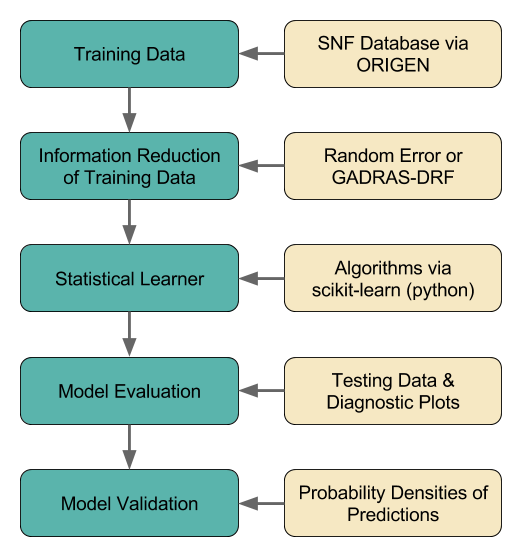
\includegraphics[width=0.9\linewidth]{./chapters/demo_method/methodology.png}
  \caption{Methodology of the proposed experiment.}
  \label{fig:method}
\end{figure}

Next, this work will expand upon the previous work in two ways.  The first is
adding a different information reduction technique via applying a gamma
spectroscopy \gls{DRF} to the \gls{SNF} nuclide recipes, which can calculate
various spectra based on the types of gamma detectors available to the
forensics community.  Secondly, a more advanced machine learning algorithm,
support vector regression, is included so as to compare more complex models
against simpler models.  A schematic of the workflow involving the experimental
components is shown in Figure \ref{fig:method}.

\section{Training Data}
\label{sec:training}

\begin{frame}
  \frametitle{Training Set}
  \begin{table}
    \centering
    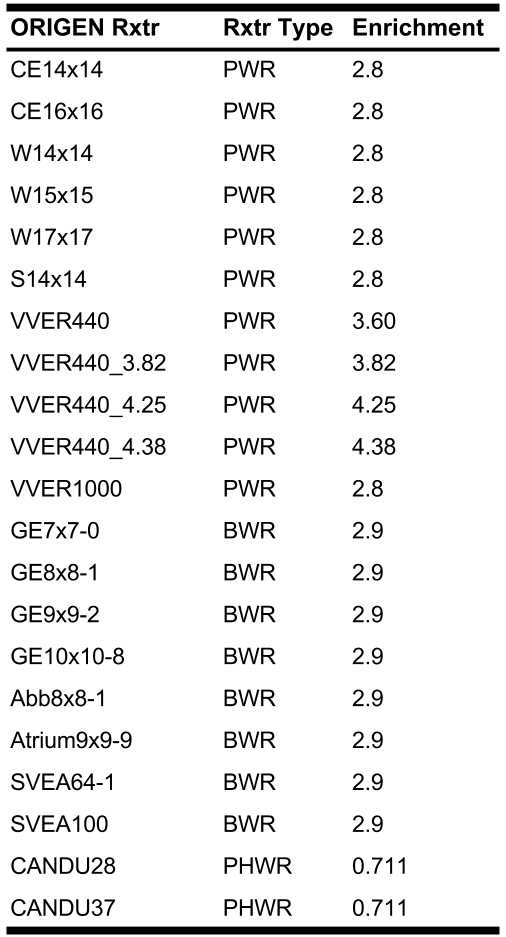
\includegraphics[height=0.9\textheight]{./figures/TrainData.png}
    \caption{caption}
  \end{table}
  \begin{table}
    \centering
    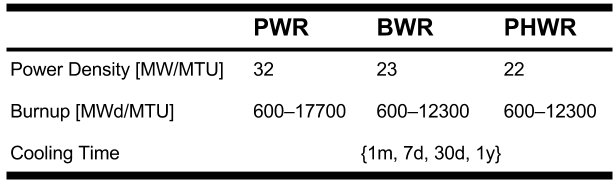
\includegraphics[height=0.9\textheight]{./figures/TrainData2.png}
    \caption{caption}
  \end{table}
\end{frame}

\begin{frame}
  \frametitle{Independent Testing Set}
  \begin{table}
    \centering
    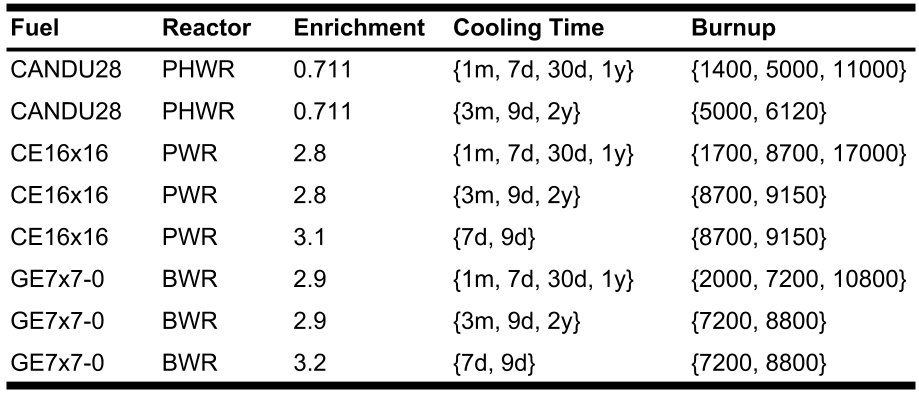
\includegraphics[height=0.9\textheight]{./figures/TestData.png}
    \caption{caption}
  \end{table} 
\end{frame}

\begin{frame}
  \frametitle{Information Reduction}
  Random error here

  gamma not implemented here
\end{frame}



\section{Statistical Learning for Models}
\label{sec:statmodel}
\subsection{Algorithms Chosen}
\label{sec:choice}

Choosing which algorithms to test is usually based on what is being predicted
and intuition regarding strengths and weaknesses of different optimization
methods.  

For a benchmarking excercise, some machine learning approaches here were chosen
based on previous work \cite{dayman_feasibility_2013}: nearest neighbor and
ridge regression. These are useful because they are simple, providing a
dissimilarity-based model and a linear regression-based model, respectively. If
more complex algorithms are not required to obtain useful results, then there
is no need to use more computationally expensive options. However, hedging on
the fact that more complex models will be needed, this work also employs an
algorithm that is known to handle highly dimensional data sets well: support
vector regression. These algorithms were introduced in Section \ref{sec:algs}. 

\begin{table}[!htb]
  \centering
  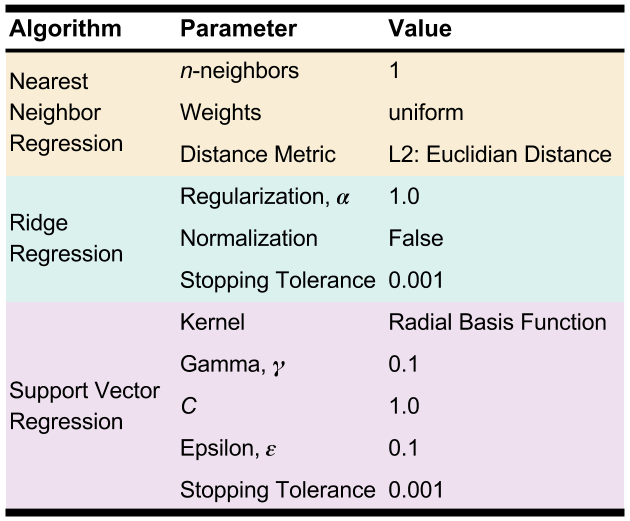
\includegraphics[width=0.8\linewidth]{./chapters/demo_method/defaults.png}
  \caption{Defaults.....................}
  \label{tbl:defaults}
\end{table}

A python-based machine learning toolkit, scikit-learn \cite{scikit}, is used to
train the models. The default parameters used for the algorithms are in
Table \ref{tbl:defaults}.

\subsection{Reactor Parameter Prediction}
\label{sec:rxtrparam}

The prediction of reactor parameters here is done with the burnup of the
\gls{SNF} to provide algorithm and corresponding model generalizability.
Following the training phase of the models, next it is important to estimate
the reactor parameter predication capabilities of those models. This is done
with a set of measurements from a test data set with samples that mimic
interdicted \gls{SNF}. The testing set has the same features as the training
set, with labels that are compared to the predicted labels. The results of each
model's prediction errors are shown in Table \ref{tbl:err}. 

\begin{table}[!htb]
  \centering
  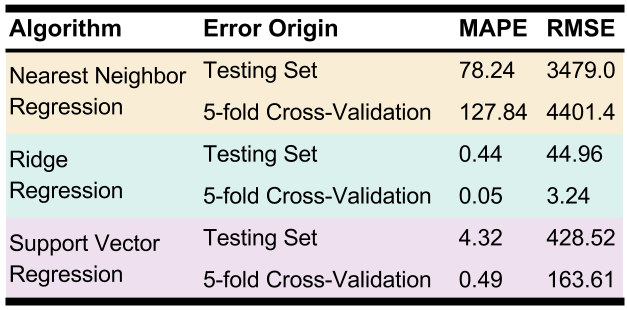
\includegraphics[width=0.8\linewidth]{./chapters/demo_method/err.png}
  \caption{Model burnup prediction errors for three algorithms}
  \label{tbl:err}
\end{table}

First shown in Table \ref{tbl:err} are testing set errors and cross-validation
errors, because although previous work uses the former, it is expected that the
latter will provide better estimates.  The models evaluated by the testing set
do not have a validation set for pre-evaluation.  The models that are evaluated
via cross-validation do not use the testing set. 

Table \ref{tbl:err} includes two error types.  For the sake of comparison to
previous work and convenient interpretation, \gls{MAPE} is tracked. However,
\gls{MAPE} requires that no true values are $0$.  The preferred method in the
community is to use \gls{RMSE} for model error estimation, so both are
tabulated.  The \gls{MAPE} shows that there are some extremely high and
extremely low errors depending on the algorithm, both of which are quite
concerning, as this indicates poor performance.  

\begin{figure}[!htb]
  \centering
  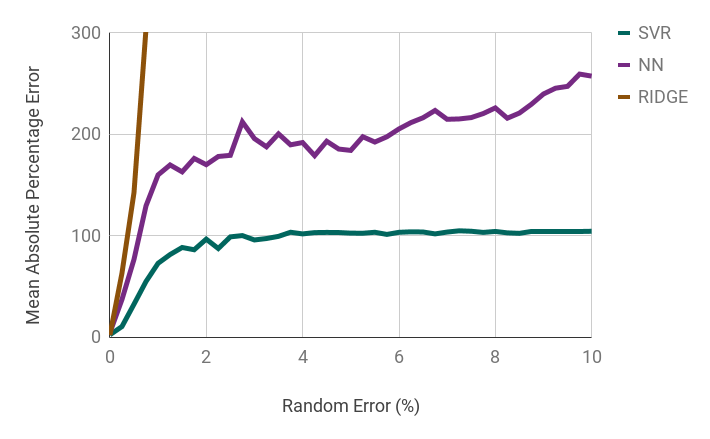
\includegraphics[width=\linewidth]{./chapters/demo_method/randerr.png}
  \caption{Results from information reduction using random error}
  \label{fig:randerr}
\end{figure}

Figure \ref{fig:randerr} shows the three algorithm's \gls{MAPE}s with respect
to the reduction of information by the introduction of random error to the
nuclide vectors as described in Section \ref{sec:inforeduc}.  \gls{SVR} is
shown to perform the best, but it quickly reaches 100\% error.  Although ridge
regression rapidly increases with any amount of error, nearest neighbor
regression shows more promise, although it reaches 257\% at 10\% error.
Overall, this performance indicates that these algorithms are unlikely to
predict burnup when faced with uncertainties in real-world measurements or
the further reduction in information from gamma detection.

Given the results in Table \ref{tbl:err} and Figure \ref{fig:randerr}, next
introduced are some diagnostic and optimization procedures that can shed light
on the performance.


\section{Validation}
\label{sec:valid}
To obtain reliable models, one must both choose or create a training set
carefully and study the impact of various algorithm parameters on the error.
Although the title of this section suggests final steps of confirming a model's
usefulness for predictions, what follows is more of a troubleshooting exercise. 
In practice, these analyses are used for both purposes.

\subsection{Model Diagnostics}
\label{sec:algeval}

Machine learning algorithms are heavily dependent on the inputs and parameters
given to them, such as training set sizes, regularization, learning rates, etc.
From the results shown in Section \ref{sec:statmodel}, it is clear there is
room for improvement.  Diagnostic plots show the errors of the predicted
burnup values to the actual burnup values with respect to some variable on the
\textit{x}-axis.  As previously introduced in Section \ref{sec:optvalid}, the
errors are compared to the training error to understand the generalization
strength with respect to training set size (learning curves) and the algorithm
parameters governing model complexity (validation curves). 

In addition to machine learning best practices, another layer of comparison is
added here.  Because it is difficult to ensure consistently representative
testing data, the accuracy of a learned model should not depend on only one
testing set.  The learned model's accuracy is better estimated by using a
validation set, or even better, \textit{k}-fold cross-validation, introduced in
Section \ref{sec:selectass}. This work includes both the testing error (using
the testing set described in Section \ref{sec:training}) and cross-validation
error. The predetermined testing set will allow for comparison against the
previous work it was obtained from \cite{dayman_feasibility_2013}, but it is
assumed that cross-validation will provide a better indication of model
performance.

\begin{figure}[!htb]
    \centering
    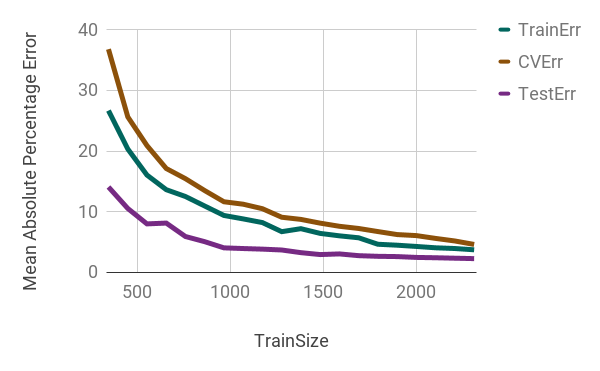
\includegraphics[width=\linewidth]{./chapters/demo_method/lc1.png}
    \caption{Learning curve for burnup prediction, $\gamma = 0.001$}
    \label{fig:lc1}
\end{figure}

The learning curves are obtained as follows, shown in Figure \ref{fig:lc1}.
For a given (randomly chosen) training set size between 15 and 100\% of the
total data set, training and prediction rounds were performed for each. The
testing error scenario performs this \textit{k} times and averages those
results.  This is equivalent to the \textit{k} in \textit{k}-fold
cross-validation to provide some semblance of equivalent statistics.  The
cross-validation error scenario has no need for averaging because it is
performed automatically. In both cases, the learning curves do not provide a
clear picture of over- or undertraining upon first glance.

\begin{figure}[!htb]
    \centering
    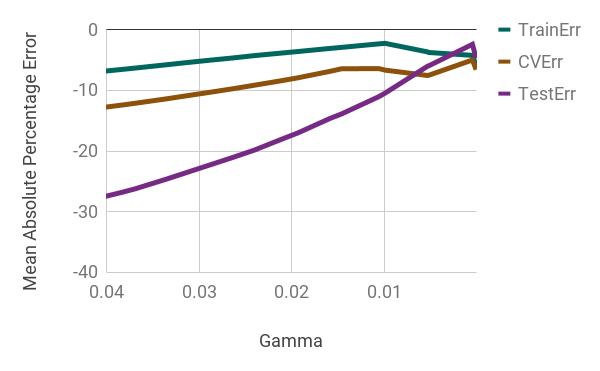
\includegraphics[width=\linewidth]{./chapters/demo_method/vc1.png}
    \caption{Validation curve for burnup prediction, $TrainSize = 2313$}
    \label{fig:vc1}
\end{figure}

The validation curves are obtained as follows, shown in Figure \ref{fig:vc1}.
The $\gamma$ parameter in \gls{SVR}, which influences model complexity, was
varied from $10^{-4}$ to $10^{-1}$. Training and prediction rounds were
performed for different $\gamma$ values in this range.  Again, the testing and
cross-validation errors are both used as described above. As with Figure
\ref{fig:lc1}, determining the robustness to over- or undertraining is
difficult here although there is possibly a minimum at $\gamma = 0.001$.

Although there is no example behavior of Figure \ref{fig:lc1}'s peculiar
learning curve in Figure \ref{fig:learning}, the curve mimics the squared bias
curve from Figure \ref{fig:bvtradeoff}. This indicates that the bias in the
model is much higher than the variance.  Next, the testing error is lower than
the training error; this should never be the case, and indicates an issue with
the systematically chosen testing set.  While the cross-validation error is
correctly higher than the training error, it follows along in parallel,
producing no information on model fitness other than confirming a very high
bias.  It is presumed this is not the fault of the algorithms, but the training
set itself.  It is likely covering too small of a range of the simulation
space.

Additionally, Figure \ref{fig:vc1}'s validation curve shows the testing error
dropping below the training error for extremely small $\gamma$, around where a
minimum might be.  Since the model suffers from high bias, no amount of model
complexity can be optimized. The resolution to the underfitting is discussed in
Section \ref{sec:prep}.

%%%%%%%%%%%%%%%%%%%%%%%%%%%%%%%%%%%%%%%%%%%%%%%%%%%%%%%%%%%%%%%%%%%%%%%%%%%%%
%%%%%%%%%%%%%%%%%%%%%%%%%%%%%%%%%%%%%%%%%%%%%%%%%%%%%%%%%%%%%%%%%%%%%%%%%%%%%
\subsection{Model Comparison}
\label{sec:algcompare}
%%%%%%%%%%%%%%%%%%%%%%%%%%%%%%%%%%%%%%%%%%%%%%%%%%%%%%%%%%%%%%%%%%%%%%%%%%%%%
%%%%%%%%%%%%%%%%%%%%%%%%%%%%%%%%%%%%%%%%%%%%%%%%%%%%%%%%%%%%%%%%%%%%%%%%%%%%%

In addition to evaluating a single learned model, it may be beneficial to
compare models.  Options for comparison of algorithms: inverse bayesian stuff,
Scatter plots, Pairwise t-tests. Confidence intervals on predictions to
understand true error versus sample error Test set must be $> 30$ instances,
Can easily calculate $N\%$ confidence interval.


